%--------------------------------------------------
%	DOCUMENT CONFIGURATION
%--------------------------------------------------
\documentclass[a4paper, 11pt, titlepage]{article}
\usepackage[utf8]{inputenc}
\usepackage[T1]{fontenc}
\usepackage[french]{babel}
\usepackage[margin=1in]{geometry}
\usepackage{amsmath, amssymb, mathtools, amsthm}
\usepackage{graphicx}
\usepackage{subfiles}
\usepackage[table]{xcolor}
\usepackage{titlesec}
\usepackage{tikz}
\usepackage{tkz-graph}
\usepackage{listings}
\usepackage{subcaption}
\usepackage[backend=biber,style=numeric,citestyle=numeric]{biblatex}
\usepackage{csquotes}
\usepackage{changepage}
\usepackage{appendix}
\usepackage{hyperref}
\usepackage{cleveref}
\usepackage{tikz-uml}
\usepackage{multicol}
\usepackage{adjustbox}
\usepackage{csvsimple}
%-----------------------------------------------
% DOCUMENT CONFIG
%-----------------------------------------------
% Add point after title number
\titleformat{\section}[block]{\sc\bfseries\center\Large}{\thesection.}{0.5em}{}
\titleformat{\subsection}[block]{\sc\bfseries\center}{\thesubsection.}{0.5em}{}
\titleformat{\subsubsection}[block]{\sc\bfseries\center}{\thesubsubsection.}{0.5em}{}
% Commands
\newcommand{\yy}[1]{\colorbox{yellow!70}{#1}}
\newcommand{\bb}[1]{\colorbox{blue!30}{#1}}
\newcommand{\rr}[1]{\colorbox{red!30}{#1}}
\newcommand{\gr}[1]{\colorbox{green!30}{#1}}
% Tikz
\tikzstyle{vertex}=[circle, draw, inner sep=2pt, minimum size=8pt]
\newcommand{\vertex}{\node[vertex]}
\usetikzlibrary{arrows,petri,topaths,calc}
% DOC INFO
\title{Rapport de Projet Tuteuré - ANDROIDE}
\author{Alexandre Bontems, Gualtiero Mottola, Hans Thirunavukarasu}
% Listings
\lstset{
frame=lines,
basicstyle=\ttfamily\small,
numbers=left,
numberstyle=\tiny,
%numbersep=5pt,
literate=%
{é}{{\'e}}1
{ê}{{\^e}}1
{à}{{\`a}}1,
commentstyle=\color{gray},
language=Octave
}
% Figures in multicols 
\newenvironment{figurecol}
  {\par\medskip\noindent\minipage{\linewidth}}
  {\endminipage\par\medskip}
% Theorems
\newtheorem{observation}{\it\bfseries Observation}
\newtheorem{definition}{\it\bfseries Définition}
%images storage 
\graphicspath{ {./images/} {./sections/images/} }
% Bibliography
\addbibresource{bibliography.bib}
%--------------------------------------------------
%	DOCUMENT BODY
%--------------------------------------------------
\begin{document}	
	\begin{center}
	    
\includegraphics[width=0.3\linewidth]{sorbonne}\\[0.8cm]
	    \textsf{\large\bfseries Rapport de Projet Tuteuré - PANDROIDE}\\[0.25cm]
	    \textsf{\Large\bfseries Pas de jaloux, un jeu de partage équitable}\\[0.5cm]
	    \textbf{Auteurs}\\
	    Alexandre Bontems\\Gualtiero Mottola\\Hans Thirunavukarasu\\[0.25cm]
	    \textbf{Superviseurs}\\
	    Nicolas Maudet\\Aurélie Beynier\\[0.5cm]
	    \textit{Université Pierre et Marie Curie, Paris 6, Département Informatique\\4 place Jussieu 75252 Paris cedex 05, France}\\[0.5cm]
	\end{center}
	\begin{adjustwidth}{.5in}{.5in}\small
	    Dans le cadre du master informatique \textsf{ANDROIDE} de l'UPMC, un projet tuteuré doit être effectué par les étudiants et ce rapport en détaille les résultats. Le problème de partage équitable LEF (Local Envy Freeness), présenté en \cite{lef}, est étudié et un jeu puzzle en est dérivé. Pour répondre aux problématiques d'analyse de difficulté pour l'humain, des résolutions \textquote{à la main} sont observées et des outils sont développés pour tenter d'expliquer les ressentis. Le développement d'une application jeu pose également les problématiques liées à l'expérience utilisateur et de conception de tutoriel. 
	\end{adjustwidth}
	\tableofcontents
%	\newpage

	\section{Introduction}
		\subfile{sections/intro.tex}
	\section{Analyse d'instances}
	    \label{sec-analyse}
        \subfile{sections/analyse.tex}
	\section{Application mobile}
	    \label{app}
	    \subfile{sections/app.tex}
	    
	\section{Travail futur}
    Un certain nombre de pistes peuvent être mentionnées pour continuer ce projet et peut être en améliorer les résultats. En effet, un travail d'observation des résolutions humaines correctement formalisé pourrait donner de nouvelles perspectives pour la conception de mesures rapide à calculer et intéressantes. Les mesures présentées dans ce rapport sont certainement améliorables également. Particulièrement la mesure \texttt{npstn} comptant le nombre de positions possibles des objets dans une instance; il serait intéressant de mesurer le processus d'élimination qui découle de ces positions. En ce qui concerne l'apprentissage, il serait bon de déterminer quelles features sont les plus intéressantes dans les modèles développés. D'autres classifiers et autres méthodes de régression sont à essayer également.
    
	L'application jeu quant à elle, bien que jouable et amusante selon certains utilisateurs, peut également faire l'objet d'améliorations. Les niveaux sont actuellement stockés en durs dans un fichier XML mais des solutions simples sont disponibles pour charger les niveaux depuis internet. Des extensions du jeu sont également à considérer comme par exemple la possibilité de changer la configuration du réseau liant les agents. On peut imaginer une action obstruant la visibilité entre deux agents et supprimant ainsi la possibilité de jalousie entre eux. Échanger les positions de deux agents côte à côte change complètement la donne du problème mais est une piste intéressante en terme de jouabilité. Enfin, seul l'écosystème Android est supporté mais une version iOS pourrait être facilement développée.
	
	\section{Conclusion}
	
	Nous avons pu proposer plusieurs outils d'analyse du problème LEF que nous espérons pertinents pour des résolutions \textquote{à la main} par des humains. Même si les résultats sont peu concluants et n'aide pas beaucoup à établir une causalité entre les mesures et les ressentis, nous croyons tout de même en l'utilité des outils. Cependant tenter de prédire une certaine rationalité des humains est peut-être vain en utilisant notre approche.
	
	Ce projet s'est révélé enrichissant sur plusieurs niveaux. Nous avons pu mettre en pratique les différentes méthodes d'optimisation et de résolution apprises au sein de notre formation. Nous plonger dans la littérature des problèmes de satisfaction de contraintes, d'optimisation combinatoire et du problème de sélection d'algorithme nous a permis d'appréhender et apprécier les différentes communautés en action. En parallèle, grâce au développement de l'application de jeu, toutes les problématiques d'ingénierie, de travail en équipe et de conception d'interface étaient des défis bienvenus. Tenter de comprendre comment la psyché humaine pouvait influer sur les résolutions était difficile pour nous, étudiants en informatique, mais encore une fois un pan de recherche particulièrement captivant. Enfin, nous avons pu gratter la surface des travaux de nos collègues DAC grâce à la partie apprentissage.
	
%	\bibliography{bibliography}
    \printbibliography[heading=bibintoc]
    
    \begin{appendix}
    \newpage
    \section{Arbre de décision}
    \label{tree}
    \begin{figure}[ht!]
        \centering
        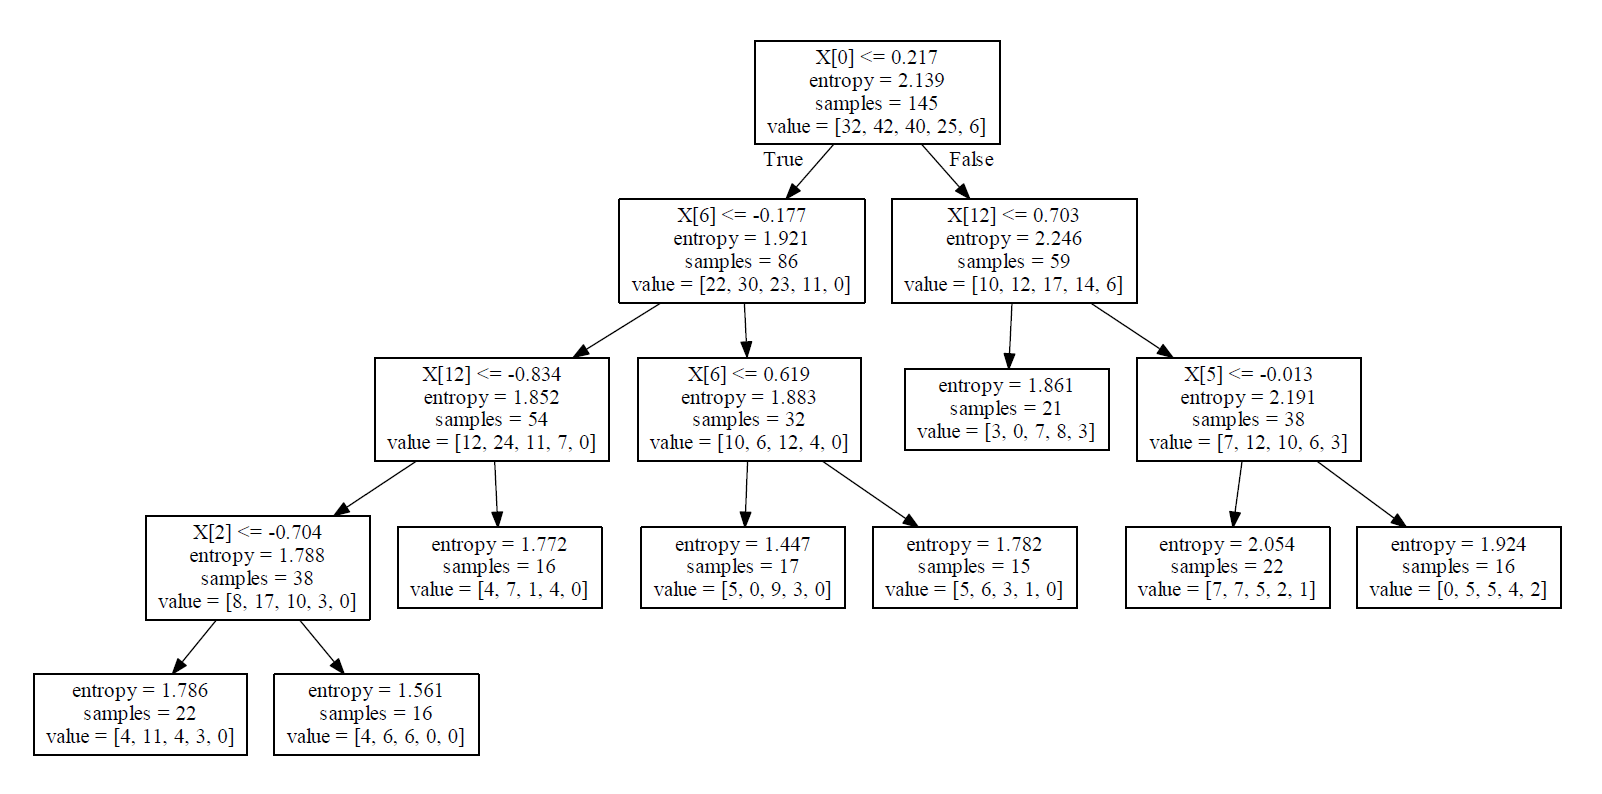
\includegraphics[scale=0.5, angle=90]{tree}
        \caption{Arbre de décision créé dans la section analyse}
    \end{figure}
    \newpage    
    \section{Tutoriel}
    Ci-après le tutoriel visible dans l'application.
    \begin{multicols}{2}
        \paragraph{1}{In this puzzle game, a number of persons are placed in a row and your goal is to choose and give a different resource to each person.
        \begin{figurecol}
        \centering
        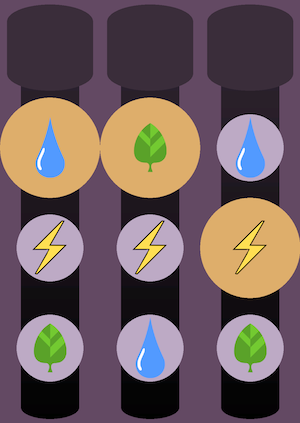
\includegraphics[width=0.8\linewidth]{tutorial1}
        \end{figurecol}
        }
        \paragraph{2}{Everyone has its own preferences concerning the resources. Those preferences are aligned in columns under each person; for example the first person on the left prefers water over power and prefers power over the leaf.}
        \paragraph{3}{The goal is to distribute those resources between our agents without creating any jealousy among them. When you assign a resource to a person, you have to be sure that the persons next to it, left side or right side, do not prefer that resource over the one they've been assigned. The same goes for the person itself.
        
    For example, we have 3 persons Alex, Bob and Charly : let's suppose you assign the water to Bob. If the resource given to Bob is in a higher position than the ones Alex or Charly have been assigned to in their preferences, they will be jealous of Bob. Here you see that Alex has the power, but he clearly prefers water over the power and sees that Bob has the water. He is therefore jealous of Bob.
    
    \begin{figurecol}
        \centering
        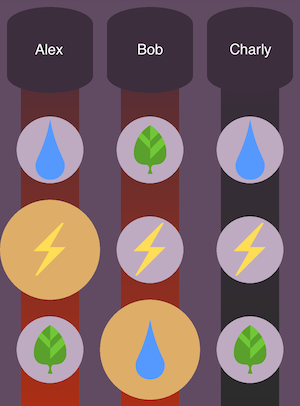
\includegraphics[width=0.8\linewidth]{tutorial2}
    \end{figurecol}
    By default, you will not be able to see which persons are envious of a neighbor but you can enable a red display for them by tapping the button \textquote{Show Envy} when playing.
    }
    \end{multicols}
    \newpage
    \section{LEF Solver}
Pour aider le développement et les tests des outils d'analyse, une application avec GUI a été développée grâce à \texttt{PyQt5} (\Cref{fig-lefsolver}). Elle permet le calcul de toutes les mesures présentées en~\Cref{sec-analyse} et de visualiser les différentes solutions trouvées par ASP. Des fonctionnalités d'exportations sont également présentes, très utiles pour l'intégration de nouveaux niveaux dans l'application pour ou pour la partie apprentissage.

\begin{figure}[ht!]
\centering
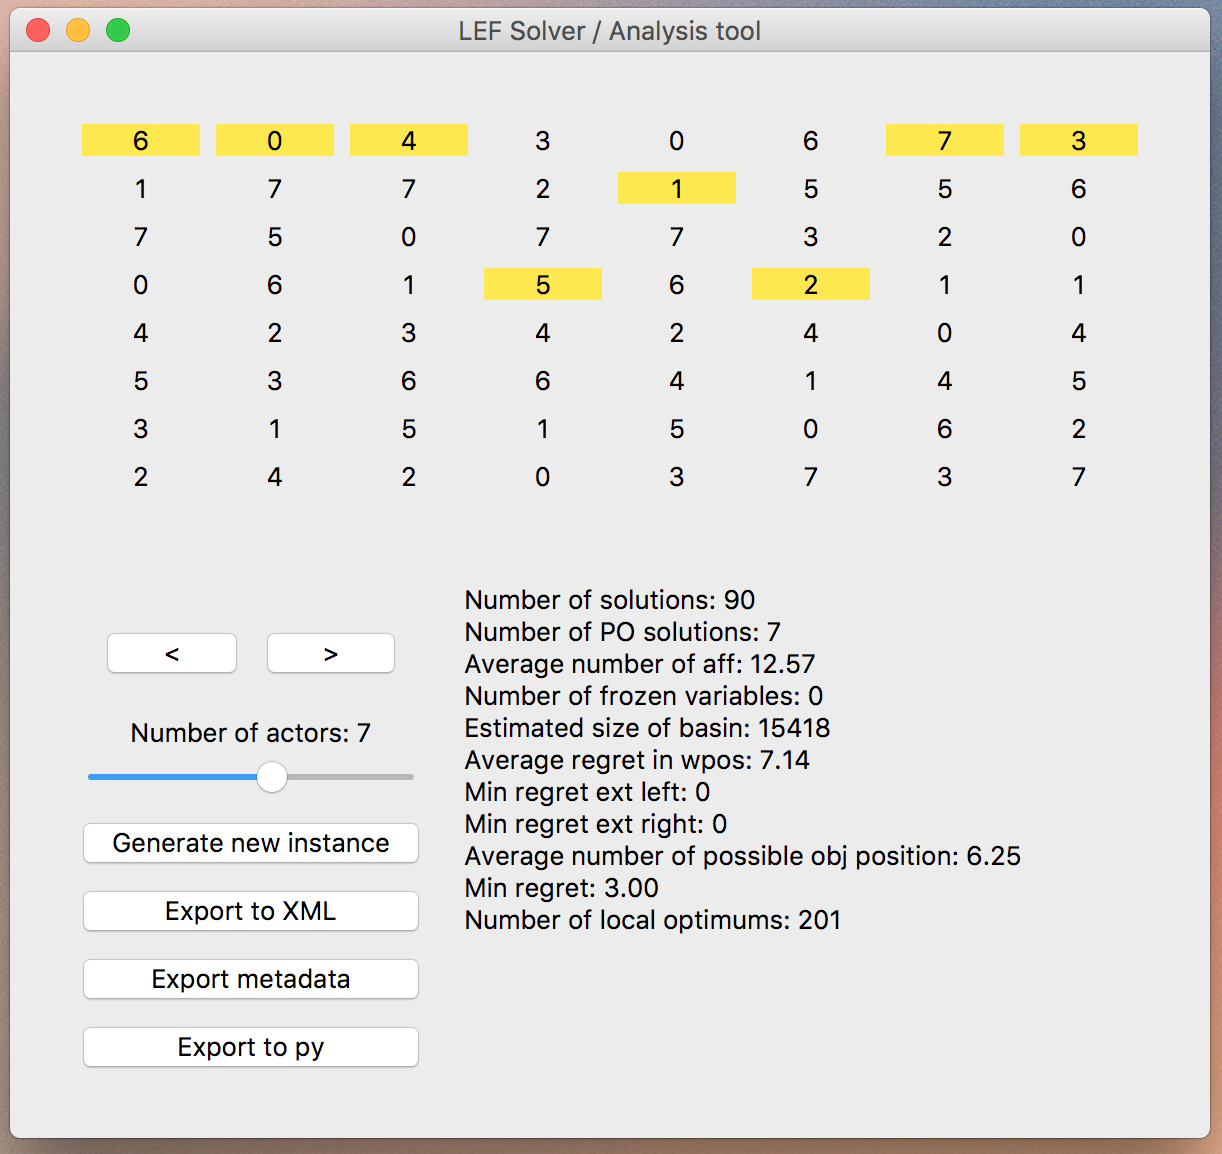
\includegraphics[width=0.7\linewidth]{lefsolver}
\caption{Capture d'écran du LEF solver}
\label{fig-lefsolver}
\end{figure}
Plusieurs actions sont possibles depuis l'unique fenêtre de cette application. Le bouton \textbf{Generate new instance} permet de générer une instance du problème solvable et de lancer les différents outils d'analyse présents dans l'application. Après résolution et analyse l'instance est affichée dans la partie haute de la fenêtre et les solutions sont exhibées en couleur jaune. Les résultats de l'analyse apparaissent également dans la partie droite.

Un slider permet de sélectionner le nombre d'agents c'est-à-dire la taille de l'instance. Des boutons fléchés donnent la possibilités de visionner toutes les solutions possibles de l'instance. Enfin les boutons d'export formatent les données relatives à l'instance et les places dans le clipboard de la machine. Le bouton \textbf{Export to XML} formate l'instance au format XML et \textbf{Export to py} au format Python c'est-à-dire une liste de dimension 2 spécifiant les ordres de préférences de chaque agent. Le bouton \textbf{Export metadata} permet de récupérer les résultats d'analyse au format CSV.
\newpage
        \section{Diagramme de classe d'Equity}
La~\Cref{fig-classdiag} montre le diagramme de classe de l'application mobile. On peut y voir les interactions entre chaque composants mais par soucis de lisibilité les méthodes et attributs ne sont pas spécifiés.
\begin{figure}[ht!]
\centering
\begin{tikzpicture}
    \umlsimpleclass{GameApplication}
    \umlsimpleclass[x=4.5]{LevelLoader}
    \umluniassoc{GameApplication}{LevelLoader}
    \begin{umlpackage}[x=8]{Models}
        \umlsimpleclass{Grid}
        \umlsimpleclass[y=-2]{Model}
        \umlassoc[mult2=1, mult1=1]{Model}{Grid}
        \umlsimpleclass[y=-4]{Level}
        \umlassoc[mult2=1, mult1=1]{Model}{Level}
        \umlsimpleinterface[x=3,y=-2]{IPiece}
        \umlassoc[mult1=1,mult2=*]{Model}{IPiece}
        \umlsimpleclass[x=2.5, y=-4]{Actor}
        \umlsimpleclass[x=5, y=-4]{Preference}
        \umlimpl{Actor}{IPiece}
        \umlimpl{Preference}{IPiece}
        \umlsimpleclass[x=4, y=-6.5]{Position}
        \umlassoc[mult1=1, mult2=1]{Actor}{Position}
        \umlassoc[mult1=1, mult2=1]{Preference}{Position}
    \end{umlpackage}
    \umluniassoc[geometry=-|-]{LevelLoader}{Level}
    \begin{umlpackage}[fill=red!20, y=-2]{Activities}
        \umlsimpleclass{MainMenuActivity}
        \umlsimpleclass[y=-1.5]{LevelMenuActivity}
        \umlassoc{MainMenuActivity}{LevelMenuActivity}
    \end{umlpackage}
    \umluniassoc[anchor2=50]{GameApplication}{Activities}
    \begin{umlpackage}[fill=red!20, y=-6]{Views}
        \umlsimpleclass{RecyclerView}
        \umlsimpleclass[x=1, y=-1.5]{GameView}
        \umluniassoc[geometry=-|-]{GameView}{Model}
    \end{umlpackage}
    \umlassoc[mult1=1, mult2=*, anchors=-35 and 35]{LevelMenuActivity}{RecyclerView}
    \umlassoc[geometry=-|-]{RecyclerView}{Level}
    \begin{umlpackage}[y=-10]{GoogleSheets}
        \umlsimpleclass{GoogleSheetsWriteUtil}
        \umlsimpleclass[y=-1.5]{SheetsServiceUtil}
        \umluniassoc{GoogleSheetsWriteUtil}{SheetsServiceUtil}
        \umlsimpleclass[x=6, type=abstract]{AsyncTask}
        \umluniassoc{GoogleSheetsWriteUtil}{AsyncTask}
        \umlsimpleclass[y=-2, x=4]{WriteUserInfo}
        \umlimpl{WriteUserInfo}{AsyncTask}
        \umlsimpleclass[y=-2, x=8]{WriteUserEvaluation}
        \umlimpl{WriteUserEvaluation}{AsyncTask}
        \umlsimpleclass[x=10]{ModifyUserProfile}
        \umlimpl{ModifyUserProfile}{AsyncTask}
    \end{umlpackage}
    \umluniassoc[geometry=-|, anchor2=70]{Activities}{GoogleSheets}
\end{tikzpicture}
\caption{Diagramme de classe non exhaustif}
\label{fig-classdiag}
\end{figure}

\newpage
\section{Cahier des Charges}
    \subsection{Présentation du projet}
    L’idée, dans ce projet, est de développer un jeu mobile basé sur le problème de partage équitable suivant:
    
\textit{n agents sont alignés sur une ligne et disposent de n objets en face d’eux. Il faut assigner un objet différent à chaque agent en fonction de leur préférence tout en prenant en compte la notion de jalousie. Si un agent voit que l’un de ses voisins (à gauche ou à droite) s’est vu attribuer un objet qu’il préfère à celui qu’il possède, alors on dira qu’il est jaloux et que l’affectation n’est pas valide.}
	
	\begin{figure}[ht!]
	    \centering
	    \begin{tikzpicture}
    	    % Agents
	        \vertex (a1) at (0,0) {$a_1$};
	        \vertex (a2) at (1.5,0) {$a_2$};
	        \vertex (a3) at (3,0) {$a_3$};
	        \vertex (a4) at (4.5,0) {$a_4$};
	        % Prefs
	        \node (a1o1) at (0,2.2) {$o_2$};
	        \node (a1o2) at (0,1.7) {\yy{$o_3$}};
	        \node (a1o3) at (0,1.2) {$o_4$};
	        \node (a1o4) at (0,0.7) {$o_1$};
	        \node (a2o1) at (1.5,2.2) {$o_2$};
	        \node (a2o2) at (1.5,1.7) {\yy{$o_4$}};
	        \node (a2o3) at (1.5,1.2) {$o_1$};
	        \node (a2o4) at (1.5,0.7) {$o_3$};
	        \node (a3o1) at (3.0,2.2) {\yy{$o_1$}};
	        \node (a3o2) at (3.0,1.7) {$o_2$};
	        \node (a3o3) at (3.0,1.2) {$o_3$};
	        \node (a3o4) at (3.0,0.7) {$o_4$};
	        \node (a4o1) at (4.5,2.2) {$o_4$};
	        \node (a4o2) at (4.5,1.7) {$o_3$};
	        \node (a4o3) at (4.5,1.2) {\yy{$o_2$}};
	        \node (a4o4) at (4.5,0.7) {$o_1$};
	        \path
	        (a1) edge (a2)
            (a2) edge (a3)
            (a3) edge (a4)	        
	        ;
	    \end{tikzpicture}
	    \caption{Exemple d'instance étudiée du problème LEF}
	    \label{fig:ex-instance}
	\end{figure}
	
	Dans l’exemple de la figure~\ref{fig:ex-instance}, les objets sont triés par ordre de préférence pour chaque agent (le plus haut étant le préféré) et une affectation possible sans jaloux est surlignée. On remarque que l'on ne peut pas affecter l'objet $o_2$ aux agents $a_1$ et $a_2$ sans créer de jalousie par exemple.
	\subsection{Objectifs}
	Ce projet s’inscrit dans le cadre de l’UE Projet du master ANDROIDE et demande de l’équipe prestataire l’application des méthodes d’optimisation apprises au sein de la formation afin de permettre l’analyse du problème exposé ci-dessus. Plus précisément, il s’agit de:
	\begin{itemize}
		\item \textbf{Déterminer la solvabilité d’une instance}.
		\item \textbf{Évaluer la difficulté de résolution d’une instance}.
		\item \textbf{Obtenir des instances de difficultés variées}.
	\end{itemize}
L’équipe prestataire est ainsi amenée à explorer des problématiques de modélisation et d’analyse de problèmes NP-difficiles avec pour objectif de trouver des heuristiques portant sur la difficulté de résolution du problème.

Dans un second temps, le développement d’un jeu mobile basé sur le problème est demandé. Les principaux résultats suivants sont attendus:
\begin{itemize}
	\item \textbf{Pouvoir jouer/résoudre une instance d’une certaine difficultée}.
	\item \textbf{Pouvoir jouer avec plusieurs instances successives selon une courbe de progression} (difficulté augmentante, variantes de jeu, etc).
\end{itemize}

\subsection{Analyse du problème}
Afin de proposer au sein de l’application des enjeux intéressants pour les joueurs, le projet devra répondre aux spécifications suivantes:
	\begin{itemize}
		\item \textbf{Obtention d’instances solvables}. 
		\item \textbf{Développement d’outils permettant d’évaluer la difficulté de résolution d’une certaine instance}. 
	\end{itemize}
On aimerait à terme intégrer les instances évaluées dans l’application mobile. Elles correspondront donc soit à des instances générées aléatoirement et qui auront pu être évaluées, soit à des instances générées procéduralement si possible. Une partie de l’analyse sera donc dédiée à la recherche des caractéristiques associées à la difficulté des instances.

Puisque les résultats sont destinés à être utilisés en tant qu'indicateurs pour une résolution par l'humain, on s'intéressera également aux méthodes de résolution du problème "à la main".

Plusieurs extensions du jeu seront considérées:
\begin{itemize}
	\item \textit{Possibilité d’échanger la position de deux agents},
	\item \textit{Possibilité d’obstruer la vision entre deux agents et donc d’éliminer toute jalousie possible entre eux},
	\item \textit{Plus d’un type d’objet possible; les agents se voient alors attribuer plus d’un objet et précisent des préférences pour chaque type différent}.
\end{itemize}

\subsection{Application Mobile}

\label{sec:app}
\subsubsection{Besoins fonctionnels: front-end}
		
L’interface de l’application mobile devra comprendre les éléments suivants:
\begin{itemize}
	\item Menu principal.
	\item Menu options.
	\item Sélection des niveaux.
	\item Écran dédié au jeu.
\end{itemize}

Elle devra aussi répondre aux problématiques principales suivantes: 
\begin{itemize}
	\item Gestion de l’encombrement de l'écran lorsque le nombre d’agents devient important; comment gérer les défilements ?
	\item Facilitation de la lecture de l’information (code couleurs, organisation de l’espace, ...).
\end{itemize}\

Afin de consolider les résultats de l’analyse, on envisage l’intégration d’une fonctionnalité de retour utilisateur pour la difficulté ressentie des niveaux. Proposer une charte graphique accueillante pour les joueurs et permettant une compréhension optimale du problème fait également partie des objectifs principaux.

\subsubsection{Besoins fonctionnels: back-end}
	
	En ce qui concerne les besoins fonctionnels de l’application, outre une architecture répondant aux spécifications front-end, il est surtout intéressant de détailler la gestion des niveaux. En fonction de l’évolution de l’analyse, deux possibilités sont envisagées:
	\begin{enumerate}
		\item Génération des niveaux sur le terminal selon des règles de générations résultantes de la première partie du projet. On pourrait ainsi offrir une grande rejouabilité.
		\item Stockage des niveaux sous forme de fichier XML qui seront alors générés et évalués en amont.
	\end{enumerate}

	Dans les premiers jours de l'application, une fonctionnalité d'enregistrement des actions utilisateurs sera inclue (dans le cadre de l'analyse des méthodes de résolution du problème par l'humain). On cherchera à extraire les intuitions qu'utilisent les joueurs pour trouver une solution et quelles caractéristiques du problèmes pourraient rendre une instance difficile face à ces intuitions.
\subsubsection{Spécifications logicielles}
	
	L’application sera développée pour la plateforme Android sous Android Studio, elle sera compatible avec tous les terminaux sous android 6.0 ou plus, la distribution du software se fera au travers de la plateforme Google Play. Le langage utilisé pour la logique de l’application sera le Java.
\subsection{Maquette de l'application}

Les figures~\ref{fig:mockup1} et~\ref{fig:mockup2} présentent un layout basique qui sera développé en profondeur lors de la phase de conception.

	\begin{figure}[h!]
		\centering
		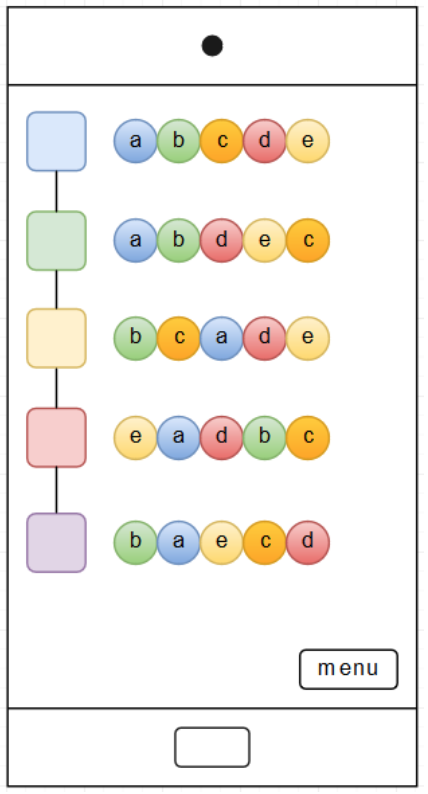
\includegraphics[width=0.3\linewidth]{maquette.png}
		\caption{Maquette conceptuelle de l'application}
		\label{fig:mockup1}
	\end{figure}
	
	\begin{figure}[h!]
		\centering
		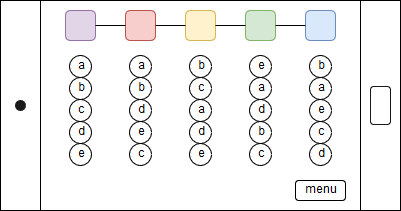
\includegraphics[width=0.7\linewidth]{maquette2.png}
		\caption{Maquette conceptuelle de l'application}
		\label{fig:mockup2}
	\end{figure}
	
\subsection{Documentation}
La production d’une documentation utilisateur est demandée. Elle concernera aussi bien toute application permettant l’évaluation des instances du problème que l’application mobile décrite en~\ref{sec:app}.
\subsection{Livrables attendus}
Les objets suivants devront être produits pour les clients:
	\begin{itemize}
		\item Documentation.
		\item Document de recherche.
		\item Sources de l’analyse.
		\item Sources de l’application mobile.
	\end{itemize}
\subsection{Planification}
\begin{center}
		\begin{tabular}{|c|c|}
			\hline
			\textbf{Livrable} & \textbf{Échéance} \\
			\hline
			Cahier des charges & 5 mars 2018 \\
			Application v0 (à faire circuler en groupe réduit) & 12 mars 2018 \\
			... & ... \\
			Rapport de projet & 25 mai 2018 \\
			\hline
			
		\end{tabular}
	\end{center}
	\newpage
	\section{Instances choisies pour apprentissage}
	\label{tab-trainset}
	\begin{table}[ht!]
		\centering
    	\small
	\begin{adjustbox}{angle=90}
	\begin{tabular}{|ccccccccccccc|}
    	\hline
    	\tt \# & \tt npo & \tt nsols & \tt avg\_naff & \tt nfrozen & \tt minr & \tt avgr & \tt minr\_extr & \tt minr\_extl & \tt npstn & \tt nlo & \tt bs & \tt ac
        \\\hline
	    \csvreader[head to column names]{inst.csv}{}
	    {\id & \npo & \nsols & \avgnaff & \nfrozen & \minr & \avgr & \minrextr & \minrextl & \npstn & \nlo & \bs & \ac\\}
%	    \hline
	\end{tabular}
	\end{adjustbox}
	\end{table}
\end{appendix}
\end{document}